\documentclass[12pt]{article}
\usepackage{amsmath, amssymb, amsthm, tikz, pgfplots}
\usepackage{geometry, enumitem, mdframed, array, xcolor}
\geometry{margin=1in}

% Custom environments
\newtheorem{definition}{Definition}
\newtheorem{theorem}{Theorem}
\newtheorem{method}{Method}
\newtheorem{example}{Example}
\newmdenv[linecolor=blue,linewidth=2pt]{keypoint}
\newmdenv[linecolor=red,linewidth=2pt]{warning}
\newmdenv[linecolor=green,linewidth=2pt]{insight}
\newmdenv[linecolor=purple,linewidth=2pt]{examtip}
\newmdenv[linecolor=cyan,linewidth=2pt]{algorithm}

\title{ODE Lesson 21: Exact Equations - Theory and Recognition}
\author{ODE 1 - Prof. Adi Ditkowski}
\date{}

\begin{document}
\maketitle

\section{Introduction to Exact Equations}

\begin{definition}[Exact Differential Equation]
A first-order differential equation of the form
\[M(x,y)dx + N(x,y)dy = 0\]
is called \textbf{exact} if there exists a function $H(x,y)$ such that
\[dH = \frac{\partial H}{\partial x}dx + \frac{\partial H}{\partial y}dy = M(x,y)dx + N(x,y)dy\]
\end{definition}

\begin{keypoint}
When an equation is exact, its solution curves are the level curves $H(x,y) = C$ of the potential function $H$.
\end{keypoint}

\section{The Exactness Criterion}

\begin{theorem}[Test for Exactness]
Let $M(x,y)$ and $N(x,y)$ have continuous partial derivatives in a simply connected domain $D$. The equation $M(x,y)dx + N(x,y)dy = 0$ is exact if and only if
\[\boxed{\frac{\partial M}{\partial y} = \frac{\partial N}{\partial x}}\]
\end{theorem}

\begin{proof}
($\Rightarrow$) If the equation is exact, then $M = \frac{\partial H}{\partial x}$ and $N = \frac{\partial H}{\partial y}$ for some $H$. By Schwarz's theorem:
\[\frac{\partial M}{\partial y} = \frac{\partial^2 H}{\partial y \partial x} = \frac{\partial^2 H}{\partial x \partial y} = \frac{\partial N}{\partial x}\]

($\Leftarrow$) The converse requires constructing $H$ from the condition, shown in Lesson 22.
\end{proof}

\section{Geometric Interpretation}

\begin{insight}
The vector field $\mathbf{F} = (M, N)$ is conservative (has a potential function) if and only if its curl vanishes:
\[\text{curl}(\mathbf{F}) = \frac{\partial N}{\partial x} - \frac{\partial M}{\partial y} = 0\]
\end{insight}

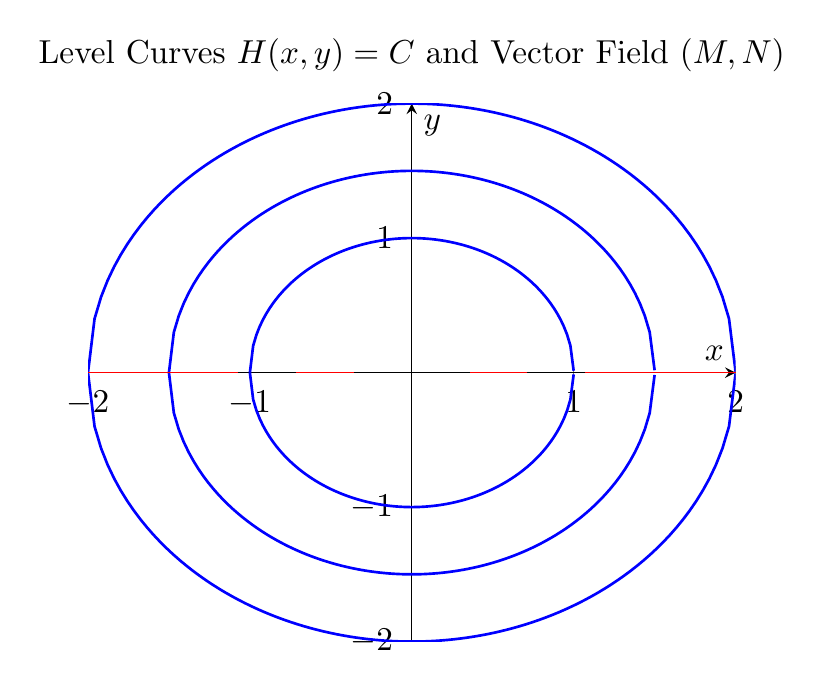
\begin{tikzpicture}[scale=1.2]
\begin{axis}[
    axis lines = center,
    xlabel = $x$,
    ylabel = $y$,
    xmin=-2, xmax=2,
    ymin=-2, ymax=2,
    title={Level Curves $H(x,y) = C$ and Vector Field $(M,N)$}
]
% Draw level curves
\addplot[blue, thick, domain=-2:2, samples=100] {sqrt(4-x^2)};
\addplot[blue, thick, domain=-2:2, samples=100] {-sqrt(4-x^2)};
\addplot[blue, thick, domain=-1.5:1.5, samples=100] {sqrt(2.25-x^2)};
\addplot[blue, thick, domain=-1.5:1.5, samples=100] {-sqrt(2.25-x^2)};
\addplot[blue, thick, domain=-1:1, samples=100] {sqrt(1-x^2)};
\addplot[blue, thick, domain=-1:1, samples=100] {-sqrt(1-x^2)};

% Draw vector field perpendicular to level curves
\addplot[red, quiver={u=-x/2, v=-y/2}, samples=8] {0};
\end{axis}
\end{tikzpicture}

\section{Connection to Physics}

\begin{keypoint}
In thermodynamics, exact differentials correspond to state functions:
\begin{itemize}
    \item Internal Energy: $dU = TdS - PdV$ (exact)
    \item Enthalpy: $dH = TdS + VdP$ (exact)
    \item Work: $\delta W = PdV$ (not exact - path dependent)
    \item Heat: $\delta Q = TdS$ (not exact - path dependent)
\end{itemize}
\end{keypoint}

\section{Algorithm for Testing Exactness}

\begin{algorithm}
\textbf{Step-by-Step Exactness Test:}
\begin{enumerate}
    \item Write equation in standard form: $M(x,y)dx + N(x,y)dy = 0$
    \item Identify $M(x,y)$ and $N(x,y)$ explicitly
    \item Compute $\frac{\partial M}{\partial y}$ (show all steps)
    \item Compute $\frac{\partial N}{\partial x}$ (show all steps)
    \item Compare the results:
    \begin{itemize}
        \item If equal $\Rightarrow$ equation is exact
        \item If not equal $\Rightarrow$ equation is not exact
    \end{itemize}
    \item State conclusion explicitly
\end{enumerate}
\end{algorithm}

\section{Common Forms and Patterns}

\begin{examtip}
Recognize these patterns that often appear in Prof. Ditkowski's exams:
\begin{enumerate}
    \item \textbf{Polynomial Forms:} $(ax^ny^m + bx^py^q)dx + (cx^ry^s + dx^ty^u)dy = 0$
    \item \textbf{Exponential Forms:} (ae^{x+y} + bx)dx + (ce^{x+y} + dy)dy = 0
    \item \textbf{Trigonometric:} $(\cos(xy) \cdot y + f(x))dx + (\cos(xy) \cdot x + g(y))dy = 0$
    \item \textbf{Mixed:} (x^2y + \sin x)dx + (x^3/3 + e^y)dy = 0
\end{enumerate}
\end{examtip}

\section{Domain Considerations}

\begin{warning}
The exactness condition guarantees existence of a potential function only in simply connected domains. Watch for:
\begin{itemize}
    \item Punctured plane: $\mathbb{R}^2 \setminus \{(0,0)\}$
    \item Domains with holes or discontinuities
    \item Multi-valued potential functions
\end{itemize}
\end{warning}

\section{Quick Reference}

\begin{keypoint}
\textbf{Memory Aid: "My Nexus"}
\begin{center}
\begin{tabular}{|c|c|}
\hline
$M_y$ & Derivative of $M$ with respect to $y$ \\
\hline
$N_x$ & Derivative of $N$ with respect to $x$ \\
\hline
\end{tabular}
\end{center}
If $M_y = N_x$, the equation is exact!
\end{keypoint}

\end{document}